%%%%%%%%%%%%%%%%%%%%%%%%%%%%%%%%%%%%%%%%%
% Stylish Article
% LaTeX Template
% Version 2.1 (1/10/15)
%
% This template has been downloaded from:
% http://www.LaTeXTemplates.com
%
% Original author:
% Mathias Legrand (legrand.mathias@gmail.com) 
% With extensive modifications by:
% Vel (vel@latextemplates.com)
%
% License:
% CC BY-NC-SA 3.0 (http://creativecommons.org/licenses/by-nc-sa/3.0/)
%
%%%%%%%%%%%%%%%%%%%%%%%%%%%%%%%%%%%%%%%%%

%----------------------------------------------------------------------------------------
%	PACKAGES AND OTHER DOCUMENT CONFIGURATIONS
%----------------------------------------------------------------------------------------
\documentclass[fleqn,11pt]{SelfArx} % Document font size and equations flushed left


%----------------------------------------------------------------------------------------
%	COLUMNS
%----------------------------------------------------------------------------------------

\setlength{\columnsep}{0.55cm} % Distance between the two columns of text
\setlength{\fboxrule}{0.75pt} % Width of the border around the abstract

%----------------------------------------------------------------------------------------
%	COLORS
%----------------------------------------------------------------------------------------

\definecolor{color1}{RGB}{0,0,90} % Color of the article title and sections
\definecolor{color2}{RGB}{0,20,20} % Color of the boxes behind the abstract and headings

%----------------------------------------------------------------------------------------
%	HYPERLINKS
%----------------------------------------------------------------------------------------

\usepackage{hyperref} % Required for hyperlinks
\hypersetup{hidelinks,colorlinks,breaklinks=true,urlcolor=color2,citecolor=color1,linkcolor=color1,bookmarksopen=false,pdftitle={Title},pdfauthor={Author}}

%----------------------------------------------------------------------------------------
%	CODES and PSEUDO CODES
%----------------------------------------------------------------------------------------

\usepackage{algorithm}
\usepackage[noend]{algpseudocode}

\usepackage{xcolor}
\usepackage{lmodern}
\usepackage{listings}
\lstset{language=[90]Fortran,
  basicstyle=\ttfamily,
  keywordstyle=\color{red},
  commentstyle=\color{blue},
  morecomment=[l]{!\ }% Comment only with space after !
}

%----------------------------------------------------------------------------------------
%	ARTICLE INFORMATION
%----------------------------------------------------------------------------------------

\JournalInfo{ Parallel Computing } % Journal information
\Archive{Development report} % Additional notes (e.g. copyright, DOI, review/research article)

\PaperTitle{Hybrid Parallelization for BATS-R-US: Adding Efficient OpenMP to MPI Code} % Article title

\Authors{Hongyang Zhou\textsuperscript{1}*} % Authors
\affiliation{\textsuperscript{1}\textit{Department of Climate and Space Sciences and Engineering, University of Michigan, Ann Arbor, MI}} % Author affiliation
%\affiliation{\textsuperscript{2}\textit{Department of Chemistry, University of Examples, London, United Kingdom}} % Author affiliation
\affiliation{*\textbf{Corresponding author}: Hongyang Zhou, hyzhou@umich.edu} % Corresponding author

\Keywords{OpenMP --- MPI --- Hybrid --- MHD} % Keywords - if you don't want any simply remove all the text between the curly brackets
\newcommand{\keywordname}{Keywords} % Defines the keywords heading name

%----------------------------------------------------------------------------------------
%	ABSTRACT
%----------------------------------------------------------------------------------------

\Abstract{We reviewed the edge-cutting finite volume MHD code Block Adaptive Tree Solarwind Roe Upwind Scheme (BATS-R-US) and managed to add coarse-grain OpenMP support to the previous pure MPI implementation, making BATS-R-US an efficient hybrid parallelization model. This paved the road for future OpenACC/Cuda development of a GPU support MHD model.}

%----------------------------------------------------------------------------------------

\begin{document}

\flushbottom % Makes all text pages the same height

\maketitle % Print the title and abstract box

\tableofcontents % Print the contents section

\thispagestyle{empty} % Removes page numbering from the first page

%----------------------------------------------------------------------------------------
%	ARTICLE CONTENTS
%----------------------------------------------------------------------------------------

\section*{Introduction} % The \section*{} command stops section numbering

\addcontentsline{toc}{section}{Introduction} % Adds this section to the table of contents

The \emph{Block Adaptive Tree Roe Upwind Scheme} (\textbf{BATS-R-US}) is an MHD code written in Fortran 90+ that  has been developed at the University of Michigan for over 20 years and is still under active development. It is at the core of the Space Weather Modeling Framework (SWMF) and has been applied to simulate multi-scale space environment phenomena including, but not limited to, solar events (coronal mass ejections, solarwind transportation), planetary global magnetosphere, comets and outer heliosphere. For the purpose of \emph{adaptive mesh refinement} (\textbf{AMR}) and running efficiency, the code was designed from the very beginning to use \emph{adaptive block} structure in 3D for parallelization. In 2012, a new \emph{Block Adaptive Tree Library} (\textbf{BATL}) is introduced for generalizing and separating the grid structure from the original source code.

However, BATS-R-US was orginally designed for pure MPI application and missed the rapid development of multi-threading technique starting from late 1990s. Even though MPI are generally observed to give better scalings than OpenMP, one obvious shortcoming of the current pure MPI implementation is memory usage: the tree structure (which will be explained in detail in the following review section) for storing the grid information as well as other precalculated variables are replicated on every MPI process, so memory leakage would happen if the number of MPI tasks used exceeds about $30000$ or the number of blocks exceeds a few million on a 2 GB/core computing node. In order to scale to more cores in the current high performance clusters, we need the aid of multi-threading and shared memory. Adding OpenMP to BATS-R-US makes it a hybrid parallel code without lossing much efficiency, while in the meantime a maximum grid size of more than an order of magnitude larger than the orginal code is achieved.

%--------------------------------------
\section{Current Code Review}

BATS-R-US was originally designed around a 3D block-adaptive grid, but it has been greatly extended in recent years. 
Each block has the same number of cells, but the blocks can have different sizes in physical space. The blocks can be split into eight children (refinement), or eight blocks can be merged into one (coarsening). Block adaptivity has a lot of advantages: each block is a simple structured grid allowing various numerical schemes, the fixed-size blocks are easy to load balance, the data corresponding to a block can easily fit into the cache, and the fixed length loops can be efficiently optimized (unrolled) by the compiler \cite{stout1997adaptive}. 

The block-adaptive grid algorithm has been improved and extended to handle arbitrary number of variables and generalized coordinates. Message passing over the poles of spherical and cylindrical grids, between cell faces edges and corners, etc., together with various algorithms, including block-to-block as well as single buffer communication, have been added to the code.

For application of block-adaptive grids with generalized coordinates in 1D, 2D and 3D, the new AMR library, i.e. \emph{Block Adaptive Tree Library} (\textbf{BATL}) is introduced as an independent part of BATS-R-US  \cite{toth2012adaptive}. It is written in Fortran 90 using the MPI library for communication, where pointers and derived types are intentionally avoided because MPI libraries available on supercomputers (at that time) lacked the capability of passing them between cores. Simple integer indexes are used instead of pointers, and arrays with named indexes instead of derived types. 

The topology of the adaptive grid can be described by a set of \emph{treenodes}. The nodes are identified by a global node index. All nodes have a bunch of information stored in an integer array \verb|Tree_IA| for tracking and organizing grid block structure. The node information (18 integers per node in 3D) is replicated on all processors, which simplifies the algorithms substantially, and it allows a lot of functionality without inter-processor communication. As long as the total number of nodes does not exceed a few million, storage should not be an issue on most supercomputers with a gigabyte or more memory per core (note that ``node'' used here is equivalent to block in BATS-R-US; it is different from a computing node on clusters). However, this drawback triggers me into thinking about using shared memory for this grid library and also the whole BATS-R-US.

The grid blocks are surrounded by $n_G$ layers of ghost cells to facilitate information exchange between the blocks. The value of the $n_G$ constant is set before compilation for the sake of efficient optimization. Numerical experiments on supercomputers are needed for the optimal true/ghost cell ratio used in simulations. 

BATL is intended to support arbitrary grid geometries, including Cartesian, spherical, cylindrical, toroidal, or even arbitrarily stretched grids. The whole computational domain is a brick in the generalized coordinates, but this can correspond to a spherical shell, a cylinder, or a distorted torus in real space. Similarly, every grid block is uniform in the generalized coordinates, but not necessarily in the Cartesian space. For the sake of efficiency useful geometrical information are precomputed : cell sizes (in generalized coordinates), face areas, face normals, cell volumes as well as the cartesian coordinates of the cell centers. This information is distributed over the processors, and it is indexed by the local block index.

For purposes of load balancing the active nodes, i.e. blocks, are ordered by a space filling curve. The root nodes are simply ordered in the usual array order by looping over them dimension by dimension. The trees starting from the root nodes are ordered recursively by looping over the children again dimension by dimension. This ordering corresponds to the Morton space filling curve. In the simplest case, load balancing means that we cut the space filling curve into $N_p$ equal pieces, where $N_p$ is the number of processors. BATL also supports a more complicated load balancing procedure, when there are different types of blocks, and each type is distributed evenly among the processors. For example the blocks on different AMR levels, or explicitly and implicitly advanced blocks can be load balanced separately. To do this the space filling curve is colored according to the block type, and then the curve of a given color is cut into $N_p$ equal pieces. In general the number of blocks per type is not an integer multiple of $N_p$, but it is ensured that the number of blocks of a given type as well as the total number of blocks per processor varies by at most 1.

With all the above features included, the high level main code structure is shown in Listing.\ref{list:code_structure}. There are 94 modules with complicated dependencies and one main file. After \verb|MPI_Init|, each process sets its own parameters , advances the solution using blocks and does the message pass every timestep through ghost cells. Being aware that most of the computation time is spent in \verb|BATS_advance| (just like all other finite volume solvers for PDEs), we focus specifically on this part of the code for modification.

From the perspective of code design, BATS-R-US follows the principle of functional programming and avoids the usage of object oriented programming. Fortran modules are used heavily for storing global variables and categorising functions and subroutines. Currently there are 99 modules in the kernel source directory, 23 in the BATL directory, and 35 in the share library. Most key variables are declared as module public variables and are called/modified upon using the specific modules.


%------------------------------------------------
\section{Hybrid Parallelization}

One of the key features of BATS-R-US is scalability on supercomputers. Previous benchmark of pure MPI results have shown good strong scaling up to 8,192 cores and weak scaling up to 16,384 cores within the memory limit. However, pure MPI parallel structure and grid-related precalculated information for efficiency generate an unavoidable memory redundancy on computational nodes. To increase the scalability to even larger sizes, we need to re-organize the code and come up with a more advanced solution beyond MPI.

The idea of hybrid programming with OpenMP and MPI arises naturally with the architecture of modern supercomputers, where each node containing several multi-core chips are connected through the network (e.g. InfiniBand). Since MPI is originally designed for distributed memory (DM) while OpenMP is designed for shared memory (SM), the initial idea of mixing them together would be to use one MPI per node and one thread per core within the node. 

There are several ways of communication supported by the current version of MPI library:
\begin{itemize}[noitemsep]
\item Single: MPI calls only outside PARALLEL regions
\item Funneled: MPI calls only on master thread
\item Serialized: MPI calls on multiple threads serially
\item Multiple: cocurrent MPI calls on multiple threads
\end{itemize}

Each of these has a specific MPI initialization indicator because of thread-safe support. For multiple-thread communication, the tags have to be used for distinguishing messages from different threads. We decided to set the support level to ``funneled'' to gain the benefits of OpenMP while minimizing the complexity of rewriting the source code. In hybrid programming, \verb|MPI_Init| should be replaced by \verb|MPI_Init_Thread| with the required and obtained support level as new additional arguments.

Basically two types of hybrid programming styles have been widely used: the fine-grained one, which uses \verb|omp parallel do| on the innermost intensive loops, and the coarse-grained one, which uses OpenMP threads on a relatively higher level to replace MPI tasks. For in our implementation of adaptive mesh refinement, this is closely related to the choice of parallelization level on either blocks or cells? As explained in detail above, BATS-R-US spreads the blocks among MPI processes and then loop through cells inside each block for calculating the face values, face fluxes and  source terms for update in each timestep. More specifically, there are a list of choices of numerical schemes (far beyond the original Roe Riemann solver) with up to fifth order accuracy, both in explicit and implicit timestepping. Simply speaking, explicit schemes loop over all the grid cells and update the solution one step forward from previous timestep, while implicit schemes solves linear equations iteratively until the system reach the tolerance level. We followed the coarse-grain parallelization idea and added OpenMP support to most if not all block-loops in both explicit and implicit  schemes available. The key structure of the code is shown in List.\ref{list:advance_code}. 

Note that:
\begin{enumerate}[noitemsep]
\item we are unable to add multi-thread to the stage loop because of data backward dependency;
\item most notable input argument to the subroutines called inside block loop is the loop index \verb|iBlock| (many other  arguments are neglected for demonstration);
\item there are a lot of \verb|if| statements in real research code with plenty of options;
\item MPI message passing is barried deep inside subroutine \verb|exchange_messages| called from module \verb|ModMessagePass|.
\end{enumerate}

Finding this sweet spot for adding multi-threading parallelization is the key in hybrid code with simple yet efficient implentation. 

In OpenMP, the most important characteristics of a variable is the range of scope. In such a large multi-module Fortran 90+ code as BATS-R-US, there are all kinds of arrays and scalars defined either globally or locally across all modules, making it nearly impossible to explicitly state each variable`s scope attribute property at the beginning of OMP parallelized loops. Therefore, I have to rely on the default treatment of variable scopes. In principle, all the variables defined in modules are shared; all the variables defined in functions and subroutines called from modules are private. However, naively doing parallelization following the OpenMP defaults will definitely cause errors since there are actually temporary and local variables defined in modules that shouldn`t be shared within different blocks. After some effort of searching and thinking, I came up with the solution of the ``notorious'' \verb|threadprivate| option: any array with a block index must be \verb|shared|, while those looping over cells and faces only must be \verb|threadprivate|; scalars are generally \verb|shared|, with a few exceptions if they are changing values inside the multi-threading parallelized region.

As a result of \verb|threadprivate| usage, I need to re-organize some of the array initialization subroutines. Threadprivate variables need to be initialized for each single thread used, while global variables must only be initialized once. 

I went through all the source codes (95 .f90 files in total) and applied the \verb|threadprivate| modification to those variables related to the explicit schemes. Unfortunately there is nothing like a threadprivate region in OpenMP, so I had to explictly list all the variables with the \verb|OMP threadprivate| constructs.


Further ideas of implementing OpenMP include adding multi-thread to message passing done in the BATL library and using nested OMP parallelized loops. The current version of message passing between blocks can be simply demonstrated in two categories:
\begin{enumerate}
\item if two spatial adjacent blocks are located on the same MPI process, make a direct copy from the physical cell values in one block into the ghost cells of the other block;
\item if two spatial adjacent blocks are located on different MPI process, unroll the quantities of physical cells, pass into a 1D array, do a MPI send/recv, and fill the ghost cell values on the receiver block in a known sequence.
\end{enumerate}

A possible improvement to the current algorithm is to add multi-thread to asynchronous MPI isend/irecv: we can parallelize the local copy in category 1 and inter-MPI copy in category 2 with one multi-thread loop, and then use multiple threads for MPI send/recv, respectively. This may require the highest level of thread safety support ``multiple'', with thread indexes used as tags. While still under progress, the idea is illustrated in pseudo code listed in List.\ref{list:BATL_code}.

\begin{algorithm}
\caption{Multi-threading in MPI message pass}\label{list:BATL_code}
\begin{algorithmic}[2]
\State !\$OMP parallel do
\For {iBlockSend=1:nBlock}
\If {iProc == iProcRecv}
\State local copy of physical values State\_VGB from iBlockSend to iBlockRecv
\Else
\State copy to send buffer bufferS\_I
\EndIf
\EndFor
\State !\$OMP end parallel do
\State !\$OMP parallel do
\For {iProcSend=0:nProc-1}
\State MPI\_Irecv(bufferS\_I, iProcSend, iThread)
\EndFor
\State !\$OMP parallel do
\For {iProcRecv=0:nProc-1}
\State MPI\_Irecv(bufferR\_I, iProcRecv, iThread)
\EndFor
\end{algorithmic}
\end{algorithm}

Besides, the nested loop idea will only be considered if the above ideas do not give satisfied scaling results. I can already imagine a mess in thread index when doing nested parallelization. Also up to this point, I intentionally skip the idea of dynamically allocated threads. More complicated things are considered only if simple ideas don`t work. The motto is always `keep it simple and stupid'.

One possible shortcoming in terms of performance is the thread generation overhead everytime we go into the \verb|advance_explicit| subroutine at each timestep. It may be better to move the start of parallelization region outside the subroutine and use \verb|!$OMP single| for the serial parts. This idea will be tested in the future.

References can be found in \cite{FortranOpenMPManual}, \cite{hybrid2013} and \cite{hybrid2017}. Many video tutorials can also be found on Youtube.


%------------------------------------------------
\section{Implementation}

There are several high level rules that we follow in improving the code:
\begin{enumerate}
\item For backward compatibility, the code should still work correctly and efficiently without OpenMP compilation flag.
\item Modification should be done as less as possible.
\end{enumerate}

Because of the complex module structure of the code and the incomplete explicit control of code behavior from OpenMP pragmas, we have to rely on the default rules and settings about the variable scopes, especially for the function and subroutine calls within the multi-threaded region.

Current standard of Fortran variable scope default rules:
\begin{enumerate}
\item Variables explicitly showing up in the \verb|omp| parallel section follow the common rules.
\item Module variables are shared.
\item Variables with save attribute are shared.
\item Variables being initialized are shared.
\item Otherwise variables are by default private.
\end{enumerate}


There are several issues that I encountered during the process.
\begin{enumerate}
\item There are many places in the code, especially in the implicit scheme, where the structure of interdependences within loops exists and prevent direct OpenMP parallelization. However, in most cases the indexes of starting blocks can be calculated directly from the grid structure, which then allows a multi-threaded parallelization on the block level.
\item The OpenMP reduction operations are needed for multi-threading in global timesteps calculation and update checking. In the time accurate simulation, a minimum timestep under stability criterion is needed for advance in time, where finding a global minimum can be speed up with multi-thread reduction; in the update check session, the maximum relative change of pressure or density may be needed for reducing timestep, where again OpenMP reduction can be applied.
\item Using Fortran modules without the \verb|ONLY| keyword inherits all the public variables and subroutines from the module, which may cause unexpected bugs in the program because of duplicate names. We avoid the unwanted behavior by always listing the public attributes and using \verb|ONLY| keyword to import variables and functions as needed.
\item The timing library we used in BATS-R-US only works for single-threaded MPI runs. This new OpenMP extension of the code requires a modification of the current library. Now we have a new subroutine which only record the timings from the master thread for each MPI process.

\item Compilers play important roles in high performance computing. In practice, finding the optimal combination of platform, machine, compiler and compiler flags requires careful testing. I used gfortran (which is actually is wrapper of gcc) on my local machine, ftn (which is actually a wrapper of ifort) on Bluewaters, and ifort on Pleiades.

\item Thread affinity is critical in achieving good performance on large clusters, but the setup may not be trivial and requires special attention to different machines.

For MPI/OpenMP hybrid codes built with SGI`s MPT library, all the OpenMP threads for the same MPI process have the same process ID. In this case, setting the \verb|MPI_DSM_DISTRIBUTE| environment variable to 1 (which is the default) causes all OpenMP threads to be pinned on the same core and the performance suffers. This default setting looks ridiculous to me, and I still don`t understand the purpose of it.

Following the recommended fix listed on NASA`s website, I set \verb|MPI_DSM_DISTRIBUTE| to 0 and use omplace for pinning instead in my job script. I also set \verb|KMP_AFFINITY| to disabled so that Intel`s thread affinity interface would not interfere with \verb|omplace|. The essence part of the batch script is listed in Listing.\ref{list:script}.

\begin{lstlisting}[caption=Sample batch script on Pleiades for hybrid runs,frame=tlrb,breaklines=true,columns=fullflexible,label={list:script}] 
#PBS -lselect=2:ncpus=16:mpiprocs=8:ompthreads=2:model=sandy
#PBS -lwalltime=1:00:00

module load comp-intel mpi-sgi/mpt

setenv MPI_DSM_DISTRIBUTE 0
setenv KMP_AFFINITY disabled

cd $PBS_O_WORKDIR

mpiexec -np 16 omplace ./BATSRUS.exe > runlog
\end{lstlisting}

On Blue Waters, thread affinity for a certain version of Intel compiler was known to bind threads created by one MPI process accidentally if they are not using Intel CPUs. (It`s actually AMD on Bluewaters). Intel seemed to fix this with the latest version of ifort.

Thread affinity is still kind of a mystery for me, and it takes time to figure out how to set it efficiently.

\item Load imbalance is always a concern when doing parallelization. OpenMP provides the programmer with several different tactics of scheduling. Due to the adaptive mesh used in BATS-R-US, the total number of allocated blocks may be larger than what is actually needed, and the sequence of blocks residing on one MPI process may be changed. For an overall good performance and avoid the small chunk size overhead, we use the default static schedule. 
\item User module provides great extensibility to BATS-R-US's existing capability. It allows users to control almost every part of the code and add new features to the kernel. However, the hybrid parallelization structure poses additional requirements to the users when designing their own module: they need to know when and how to do MPI communication as well as avoid false sharing and race conditions for OpenMP. The rules listed in ??? serves as an guideline for future code extensions.
\item In many scenarios, using OpenMP may not be a good idea for performance. For instance, message pass between faces is used together with grid resolution changes to conserve face fluxes in our finite volume scheme.  This usually includes too few blocks so it makes less sense to parallelize this part with OpenMP.
\end{enumerate}


%--------------------------------
\subsection{Improvements}

\subsubsection{Single fluid performance}
The multi-fluid module is introduced into BATS-R-US several years ago. The extension from single fluid MHD to multi-fluid MHD causes performance penalty for single fluid runs because of unncessary string copies and function calls for setting up the state for different fluid species. This part is now being optimized to give a $40\%$ improvement on single fluid simulations.

\subsubsection{Message passing}
The orginal message passing is done inside the BATL library for both cellwise and facewise message exchange between layers of ghost cells and neighboring physical cells. Message passing on the faces are implemented for the adaptive grid where the numerical fluxes need to be conserved between the coarse and fine cell faces on different resolution level. For all the current real applications, this part usually takes insignificant amount of time, so OpenMP pragmas are not added as the overhead may even be detrimental to performance. In the case of cellwise message passing, the old scheme combines the local exchange (message passing between blocks on the same processor) and the remote exchange (message passing between blocks on the remote processors). This turns out to be a tough case for adding multi-threading parallelization, which is now rewritten to fully separate the local and remote part. The local copies are multi-threaded while the remote exchange are done using 1D buffers and MPI iSend/iRecv. Currently this implementation only requires the thread safety level up to \verb|MPI_THREAD_FUNNELED|, which means only the main thread can make MPI calls. If we observe a significant slowdown for the MPI message passing in any future application, higher thread levels with more complex communication scheme can be tested.


\subsubsection{Preventing temporary arrays}
Temporary arrays are created when we try to pass slices of a large array which are strided in memory into another function or subroutine. This potentially slows down the code. We avoid temporary arrays in most cases by allocating local arrays and pass as assumed shape array.

\subsubsection{Parameters setup}

Because of the integrity of all kinds of numerical methods for solving the face flux for the Riemann problem, each parameter is set individually without interferences with each other for the flexibility of adding new schemes. However, the old FaceFlux module sets all the parameters during each timestep, which is modified to be done only once in the initial timestep to avoid redundant computation.


%------------------------------------------------
\section{Test and Verification}

\subsection{Platform Information}
All the testing platforms are listed in Table ???.

The verification tests are done on MacbookPro 2015 with 2.2GHz qual-core Intel Core i7 using Nagfor and gfortran compilers.

Stampede2 SKX nodes with 192 GB of memory per node. Each node contains 48 Intel Xeon Platinum 8160 Skylake cores. 

The large scale tests are done on Blue Waters Cray XE6 nodes with $64$ GB of memory per node. Each node contains 16 Bulldozer Cores with 2 AMD 6276 Interlagos Processors. There are 32 integer scheduling units per node with $2$ GB memory per unit.




\subsection{Verification}
The first series of tests were done locally with 2.2GHz qual-core Intel Core i7. These tests are the standard tests created for BATS-R-US for verification. Without any surprise, among all 46 tests designed for BATS-R-US (Table.\ref{tab:night_test}), when I compiled with OpenMP flags and used 2 threads for each MPI process, only 10 passed successfully (with a checkmark \checkmark), 6 showed differences in the outputs (with a question mark ?), and the rest caused runtime errors when running with more than 2 threads (shown with a cross \text{\sffamily X}). This shows that:
\begin{enumerate}[noitemsep]
\item The modified code works for purely explicit scheme with no AMR. Since I made no changes in the semi-implicit, point-implicit and fully implicit scheme modules, nearly all the related tests caused runtime error.
\item The pure explicit scheme only covers a small range of applications. 
\end{enumerate}

% This list may be miscounting!
\begin{table}[htbp]
  \centering
  \caption{BATSRUS nightly tests}
    \begin{tabular}{lc}
    \toprule
    Test Name & Status  \\
    \midrule
    2bodyplot & \checkmark \\
    amr & ? \\
    anisotropic & \checkmark   \\
    awsomfluids  & \text{\sffamily X}  \\
    chromo  & \checkmark  \\ 
    comet & \checkmark \\
    cometCGfluids & \checkmark \\
    cometfluids\_restart &\text{\sffamily X}  \\
    cometCGhd & \checkmark \\
    cometfluids & \text{\sffamily X} \\
    corona &\checkmark \\
    coronasph &\checkmark \\
    earthsph & \checkmark \\
    eosgodunov &\text{\sffamily X} \\
    fivemoment\_alfven &\checkmark \\
    fivemoment\_langmuir & \checkmark \\
    fivemoment\_shock &\checkmark \\
    fluxemergence & \text{\sffamily X}\\
    func & ? \\
    ganymede & \checkmark\\
    graydiffusion & \checkmark \\
    hallmhd & \checkmark \\
    laserpackage & \text{\sffamily X}\\
    magnetometer & \text{\sffamily X}\\
    mars &\checkmark \\
    mars\_restart &\checkmark \\
    marsfluids & \checkmark\\
    marsfluids\_restart &\checkmark \\
    mercurysph & \checkmark \\
    mhdions &\checkmark \\
    mhdnoncons & \checkmark \\
    multifluid & \checkmark \\
    multiion &\checkmark \\
    outerhelio & \checkmark \\
    partsteady & \checkmark \\
    region2d & \checkmark \\
    saturn &\checkmark \\
    shockramp & \checkmark \\
    shocktube & \checkmark \\
    spectrum &\text{\sffamily X} \\
    titan &\checkmark \\
    titan\_restart &\checkmark \\
    twofluidmhd &\checkmark\\
    venus &\checkmark \\
    venus\_restart & \checkmark\\
    viscosity & \checkmark\\
    \bottomrule
    \end{tabular}
  \label{tab:night_test}
\end{table}

Nevertheless, this is already impressive to me considering the minor modification ratio of the code.

Then I proceeded to do performance tests locally. The standard shocktube test and two another simple density wave propagation tests are selected to estimate the timing on my local machine with 4-core 2.2 GHz Intel i7 processor. The results are shown in Fig.\ref{fig:local_timing}. Note that this is total runtime, including the \verb|set_parameter| section (pure MPI), \verb|advance| section (MPI + OpenMP), and \verb|save_output| section (pure MPI), so we would expect a slightly decrease in overall performance for cases where $nProc * nThread = constant$ (because within one MPI process, the reading and writing parts are ``serial'' in hybrid programming sense). In addition, the \verb|threadprivate| declaration generates non-neglibile overhead to the multi-threaded region.

\begin{figure*}[htbp]
\centering
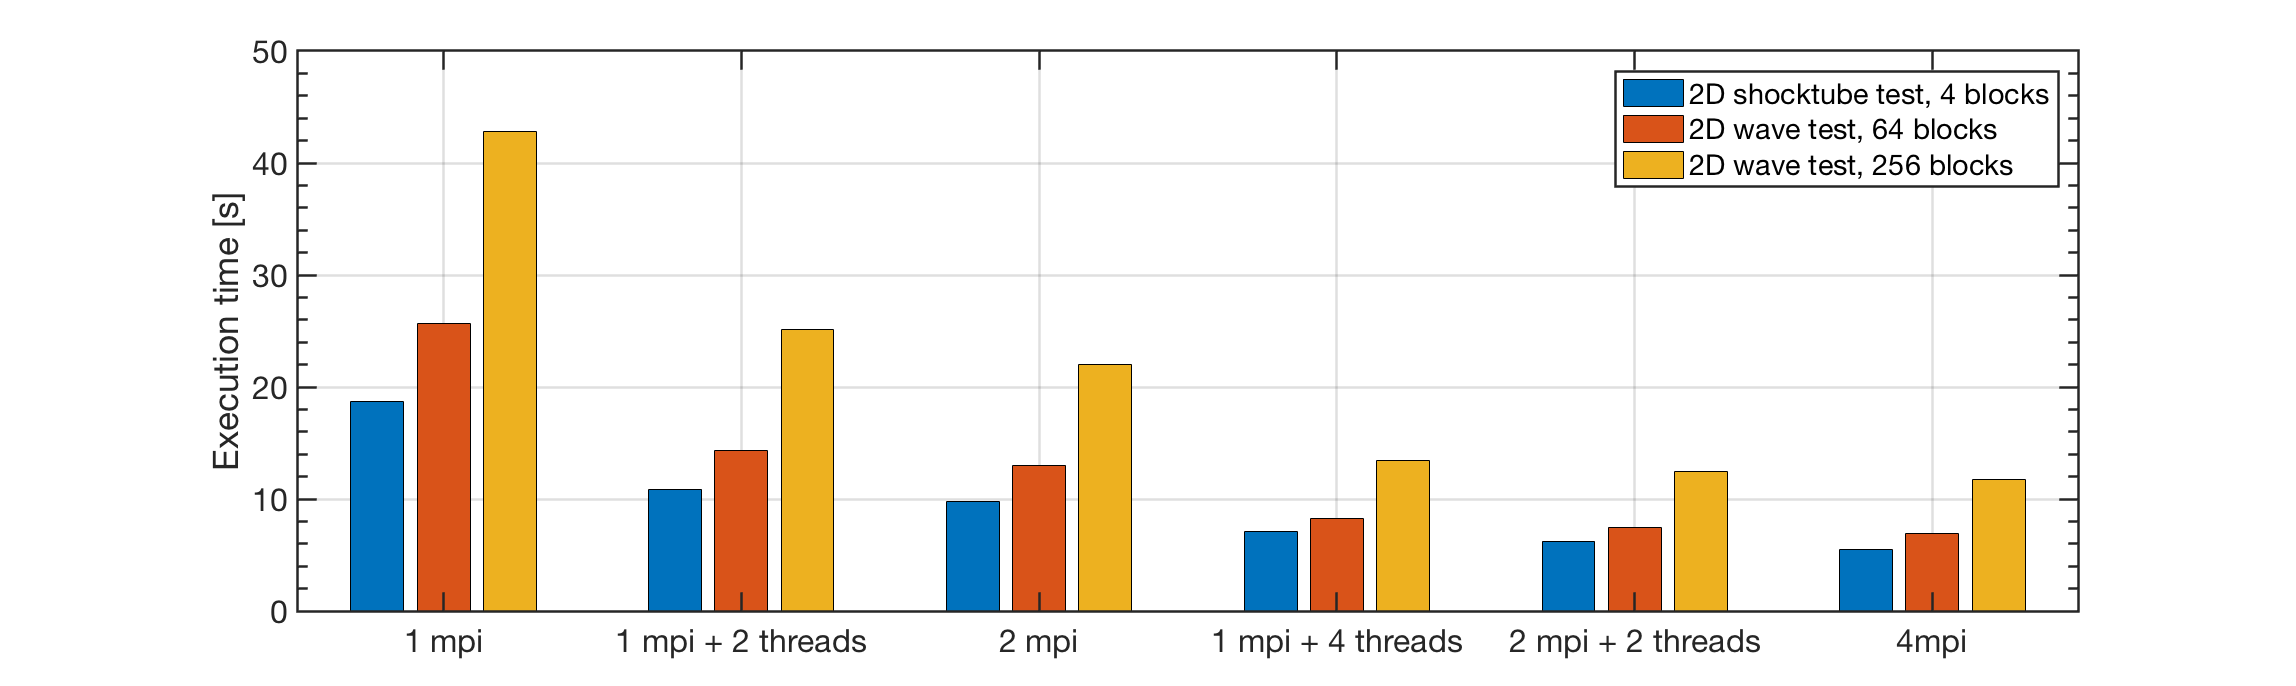
\includegraphics[width=\textwidth]{figures/local_timing}
\caption{Timing of 3 simple tests on Macbook Pro with 4-core 2.2 GHz Intel i7 processor.}
\label{fig:local_timing}
\end{figure*}


The third series of tests were done on Pleiades Sandy Bridge nodes (Fig.\ref{fig:sandy}). Each node has a dual-socket 16 core structure. In this test I use 512 blocks (8 in each dimension), with a cell size of $8*8*8$ and 2 levels of ghost cells in Cartesian coordinates. Theoretically, load balance of blocks among processors won`t be an issue in this test. Ideally, for the series of tests with mixed set of number of processors and number of threads under a fixed product ($nProc*nThread=\textrm{const.}$), we would expect a horizontal colored line if MPI and OpenMP provide perfect parallelizations. In real tests shown in Fig.\ref{fig:sandy_timing}, I observed slightly decreasing efficiency as the number of threads generated per node increases from 1 to 8, followed with a surprising drop in performance when running with 16 threads (which is equal to the number of cores on Sandy Bridge) per node. To further diagnose the problem, I went to Ivy Bridge with 20 cores per node and found the similar trend: the performance vastly decreased when the number of threads goes beyond half number of cores per node. My hypothesis is that since each node on Sandy Bridge or Ivy Bridge actually consists of 2 NUMA nodes, the thread affinity setup may limit multi-threading to one NUMA node, such that if I allocate more threads, they just fight for the physical cores and memory which results in huge decrease in timing. I believe this can be solved with more detailed explicit thread affinity setup, but for now I just leave it for the future development plan.  

\begin{figure}[htbp]
\centering
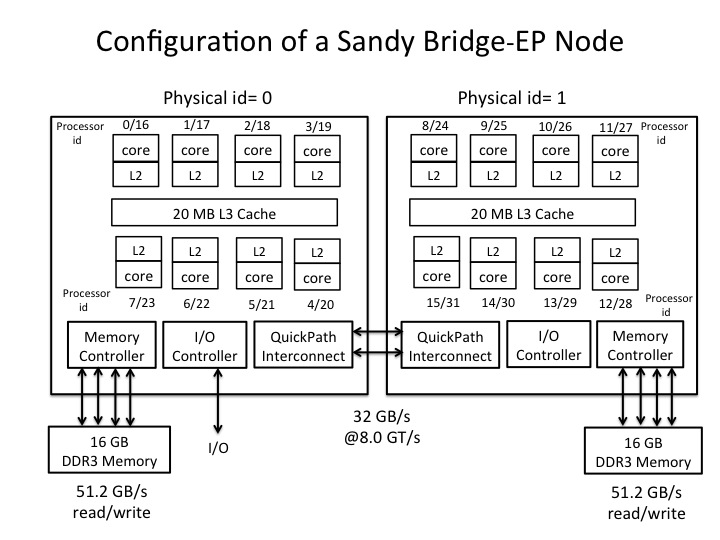
\includegraphics[width=0.5\textwidth]{figures/sandybridge_processor_numbering}
\caption{Configuration of testing node.}
\label{fig:sandy}
\end{figure}

\begin{figure}[htbp]
\centering
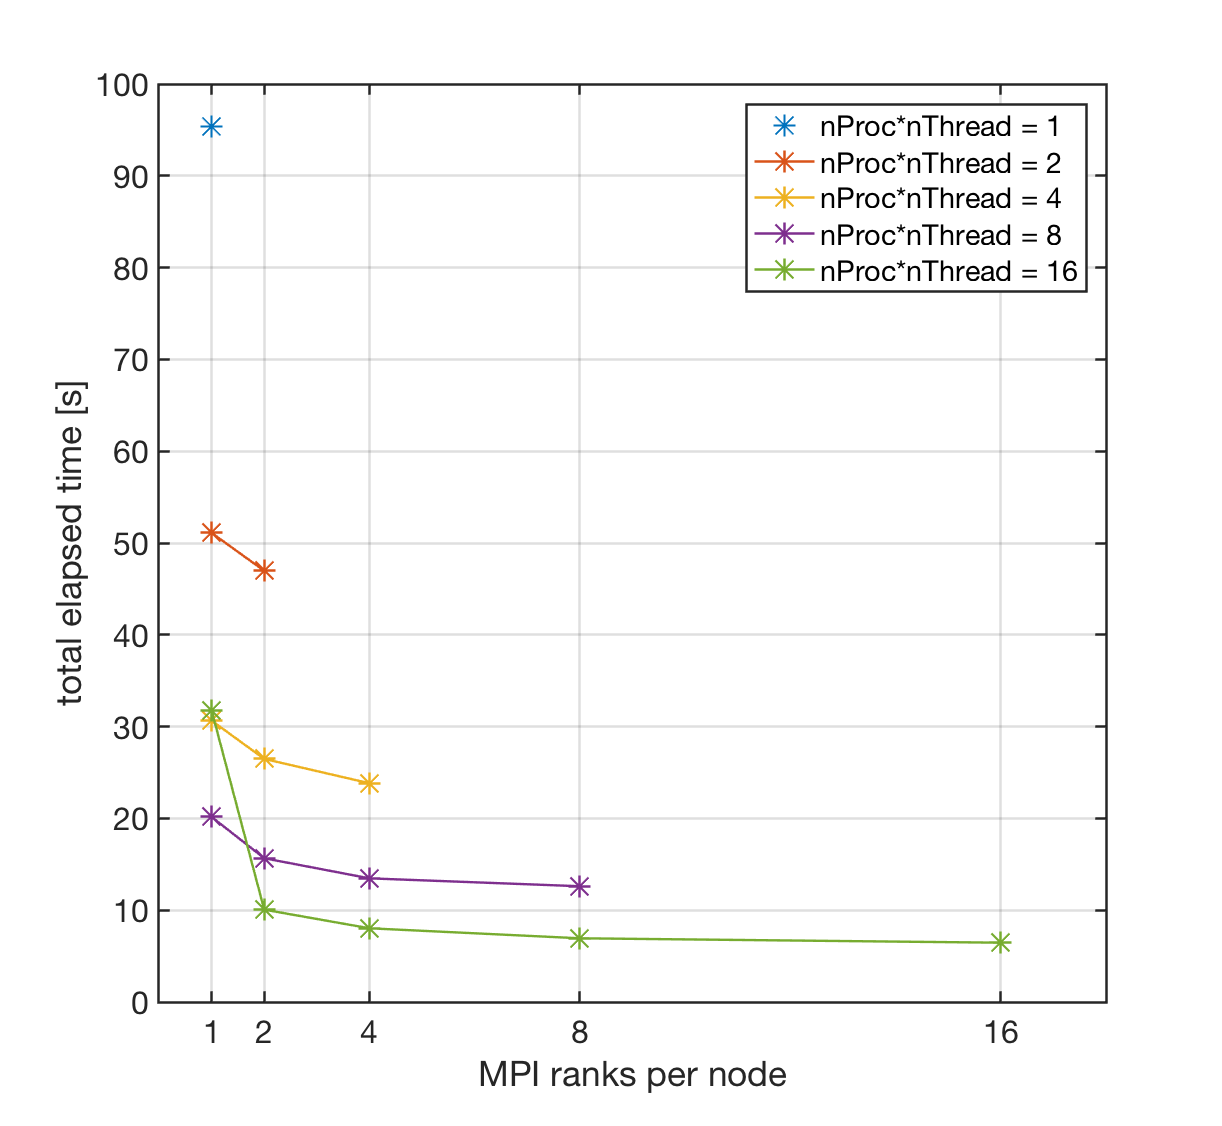
\includegraphics[width=0.5\textwidth]{figures/sandybridge_timing}
\caption{Performance on a single node on Pleiades Sandy Bridge tested with 3D wave propagation. The cell size is $8*8*8$ in Cartesian coordinates, with 2 levels of ghost cells in each dimension. The x axis represents the number of MPI processes per node, and y axis is the total elasped time. The same color represents series of runs with a fixed number of the product of $nProc$ and $nThread$.}
\label{fig:sandy_timing}
\end{figure}

The results of simple strong scaling multi-threaded test runs are shown in Fig.\ref{fig:thread_scaling} (1 MPI + multi-threads). I can get pretty good scaling up to 8 threads with an efficieny $s=0.86$. 

\begin{figure*}
\centering
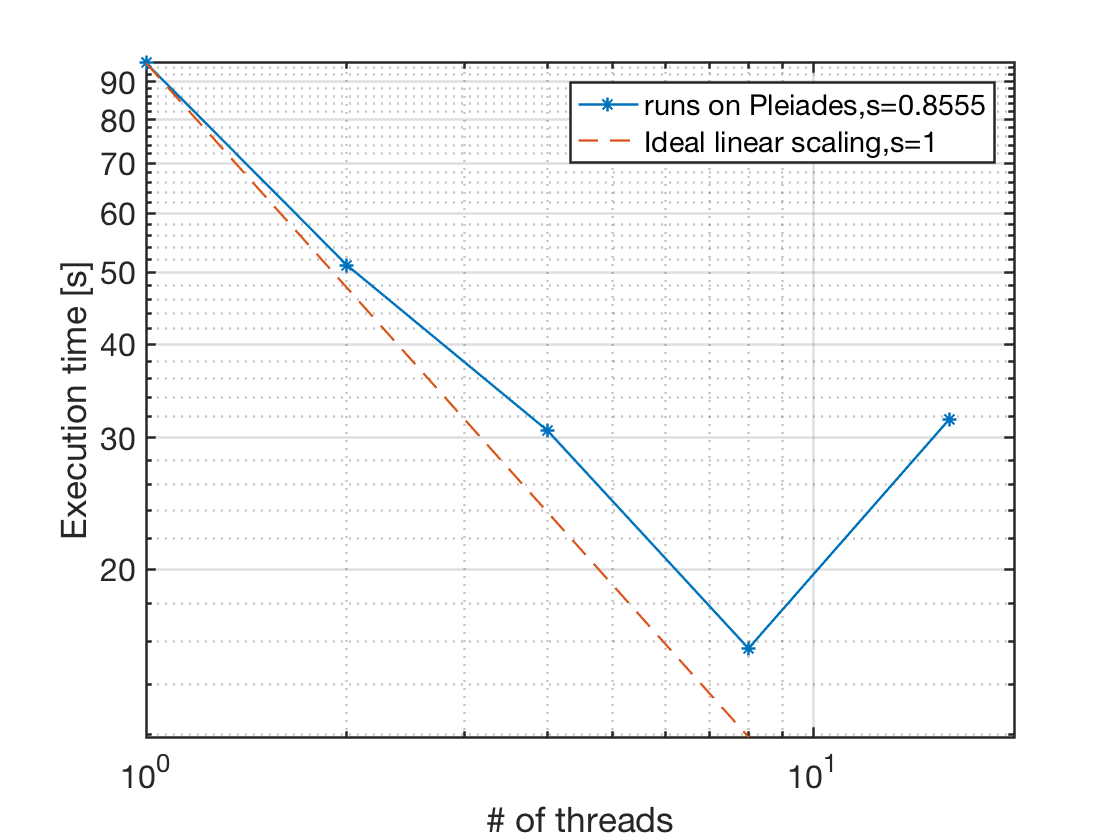
\includegraphics[width=\textwidth]{figures/thread_scaling}
\caption{Scaling with the number of threads.}
\label{fig:thread_scaling}
\end{figure*}

Another important question is whether or not I observe improved memory usage. The real memory used in hybrid simulations with $nProc*nThread=8$ is plotted in Fig.\ref{fig:memory}. I do see a significant drop in memory usage from over $600$ MB to $300$ MB from pure MPI to pure OpenMP. This illustrates the importance of shared memory usage for simulations, especially when pure MPI implementation encounters memory issue. This encouraging result gives me confidence in the upcoming large scale tests. (Based on the discussion with Gabor, this information is in fact misleading. I reduction in memory usage is mostly from the decrease in MPI processes: there`s a fixed number of blocks on each process, whether it is used or not. As long as the number of blocks is small, you cannot actually see the benefits of OpenMP!)

\begin{figure*}
\centering
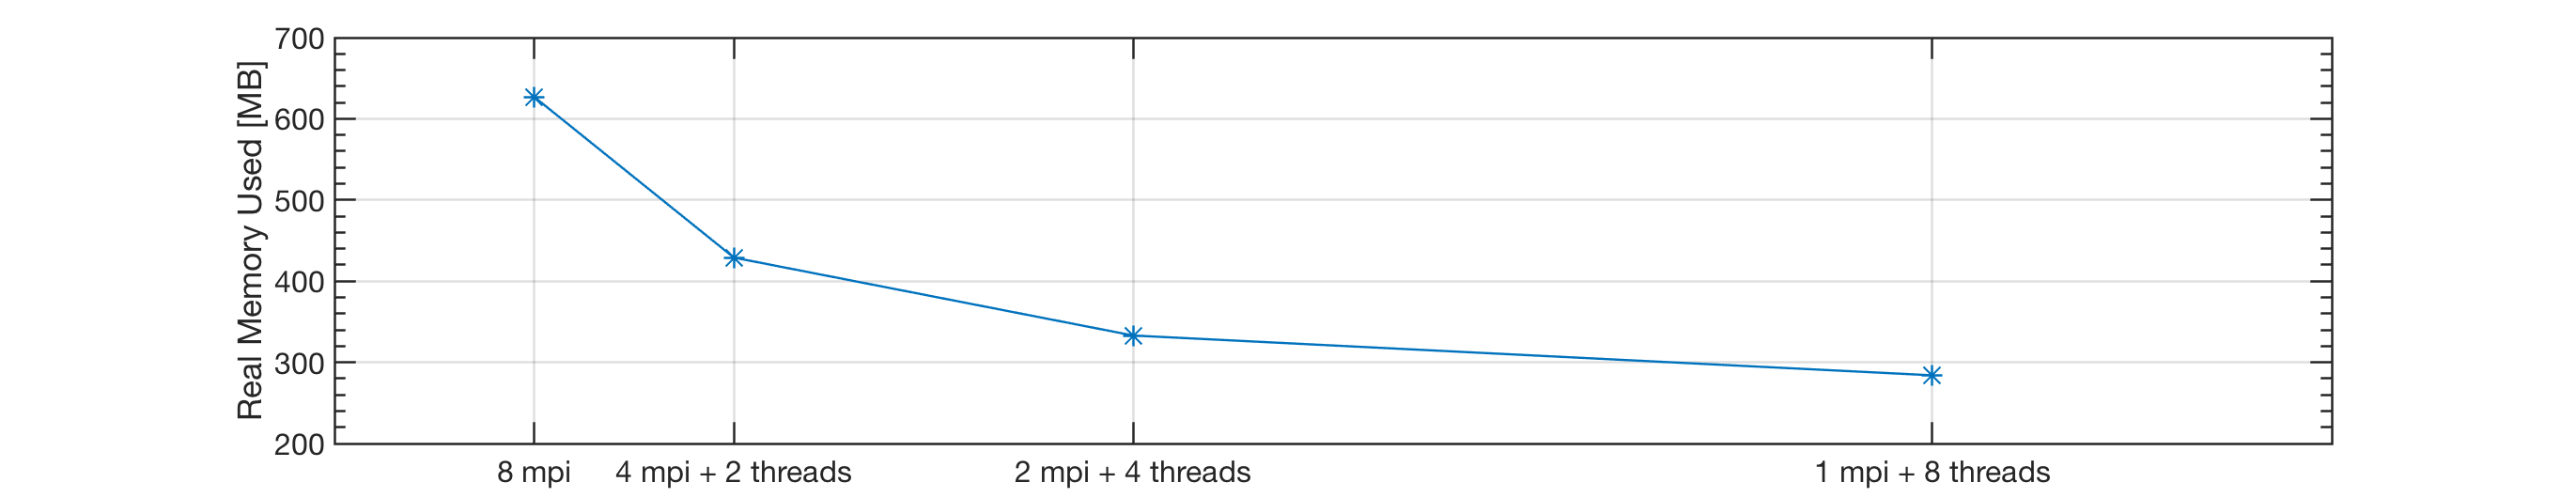
\includegraphics[width=\textwidth]{figures/memory_usage}
\caption{Memory usage for 3D wave tests monitored by system log file.}
\label{fig:memory}
\end{figure*}


%------------------------------------------------
\section{Conclusion and Future Work}
We have successfully extended our finite volume MHD code BATS-R-US with adaptive mesh refinement in general coordinates from pure MPI to MPI+OpenMP implementation. While maintaining the nice scaling performance up to $\sim 10^6$ cores, we are now able to solve problems more than an order of magnitude larger than before thanks to the usage of shared memory.
This also paves the way for porting the complex solver to accelerators and GPUs with minimum code modifications possible. 


%----------------------------------------------------------------------------------------
%	REFERENCE LIST
%----------------------------------------------------------------------------------------
\phantomsection
\bibliographystyle{unsrt}
\bibliography{sample}

%----------------------------------------------------------------------------------------

\end{document}